\documentclass[border=2pt]{standalone}

%% Fonts
%\usepackage{fontspec}
%% Default Features
%\defaultfontfeatures{
%	Mapping=tex-text,
%	Ligatures=TeX,
%}
%% Serif Font
%\setmainfont[
%	UprightFont=EBGaramond-Regular,
%	ItalicFont=EBGaramond-Italic,
%	BoldFont=EBGaramond-Bold,
%	BoldItalicFont=EBGaramond-BoldItalic,
%]{EB Garamond}
%% Mono Font
%\setmonofont[
%	UprightFont=JetBrainsMonoNL-Regular,
%	ItalicFont=JetBrainsMonoNL-Italic,
%	BoldFont=JetBrainsMonoNL-Bold,
%	BoldItalicFont=JetBrainsMonoNL-BoldItalic,
%]
%{JetBrains Mono}

% Tikz
\usepackage{tikz}
\usetikzlibrary{calc, positioning, shapes}

% Colors
%\definecolor{myyellow}{RGB}{255, 255, 191}
%\definecolor{mygreen}{RGB}{171, 221, 164}
%\definecolor{myblue}{RGB}{216, 225, 246}
% Dimensions
\def\deltadimclient{0.1}
\def\deltadimserver{0.2}
\def\padding{0.4cm}
\def\cornerradius{0.2cm}
\def\logentrieslinewidth{0.7pt}
\def\innersep{6pt}
\def\outersep{2pt}
% Client
\def\numclients{3}
\def\clientdrawcolor{gray!60!black}
\def\clientfillcolor{gray!25}
% Server
\def\numservers{4}
\def\serverdrawcolor{\clientdrawcolor}
\def\serverfillcolor{\clientfillcolor}
\def\serverheight{5.7cm}
\def\serverwidth{6.5cm}
% Replicated
\def\replicateddrawcolor{green!70!black}
\def\replicatedfillcolor{green!20}
% Entries
\def\logentriesdrawcolor{cyan!100}
\def\logentriesfillcolor{cyan!20}
\def\entriesheight{15pt}
\def\entrieswidth{34pt}
\def\textspace{2mm}
% Data Store
\def\datastoredrawcolor{orange!80!black}
\def\datastorefillcolor{orange!60}
\def\datastoreheight{9pt}
\def\datastorewidth{18pt}
% Connections
\def\connectionshift{0.35}
\def\labelinnersep{1.5pt}

% Styles
\tikzset{
	% labels
	label/.style={
		font=\footnotesize\ttfamily,
		align=center,
	},
	% node labels
	node_label/.style={
		draw,
		thick,
		inner sep=\labelinnersep,
		shape=circle,
		align=center,
	},
	% general
	module/.style={
		draw,
		very thick,
		label,
		outer sep=\outersep,
		rounded corners=\cornerradius,
		shape=rectangle,
	},
	% client
	client/.style={
		module,
		draw=\clientdrawcolor,
		fill=\clientfillcolor,
		inner xsep=\innersep,
		inner ysep=\innersep,	
	},
	% server
	server/.style={
		module,
		draw=\serverdrawcolor,
		fill=\serverfillcolor,
		minimum height=\serverheight,
		minimum width=\serverwidth,
	},
	% replicated 
	replicated/.style={
		module,
		draw=\replicateddrawcolor,
		fill=\replicatedfillcolor,
		inner sep = \innersep,
	},
	% log and state machine entries
	entries/.style={
		shape=rectangle,
		draw=\logentriesdrawcolor,
		line width=\logentrieslinewidth,
		fill=\logentriesfillcolor,
		rounded corners=0cm,
		minimum height=\entriesheight,
		minimum width=\entrieswidth,
		inner ysep=0pt,
		inner xsep=\innersep/2,
		outer sep=0pt,
	},
	% data store
	data_store/.style={
		draw=\datastoredrawcolor,
		fill=\datastorefillcolor,
		thick,
		ellipse,
		inner sep=0,
		minimum height=\datastoreheight,
		minimum width=\datastorewidth,
	},
	% connections
	connection/.style={
		thick,
		-stealth,
	}
}

\begin{document}
	\begin{tikzpicture}
		% Server
		\foreach \i in {1,...,\numservers} {
			\pgfmathsetmacro{\displacement}{\i * \deltadimserver}
			\node[
				server,
				anchor = west,
			] (server\i) at (-\displacement, \displacement) {};
		}
		%% Label
		\node[
			label,
			anchor=north west,
			shift={(\padding,-\padding)},
		] at (server\numservers.north west){server};
		
		% Log
		\node[
			replicated,
			anchor = south west,
			shift={(\padding,\padding)},
		] (log) at (server\numservers.south west) {%
			log
			%
			\\[\textspace]
			%
			\begin{tikzpicture}
				\node[
					entries
				] (log1) {$x \leftarrow 3$};
				%
				\node[
					entries,
					anchor=west,
					xshift=-\logentrieslinewidth
				] (log2) at (log1.east) {$y \leftarrow 7$};
				%
				\node[
					entries,
					anchor=west,
					xshift=-\logentrieslinewidth
				] (log3) at (log2.east) {$y \leftarrow 9$};
				%
				\node[
					entries,
					anchor=west,
					xshift=-\logentrieslinewidth
				] (log4) at (log3.east) {$\cdots$};
			\end{tikzpicture}%
		};
		%% Data store
		\foreach \i in {0,...,2} {
			\node[
				data_store,
				shift={(\datastorewidth/6,\i * \datastoreheight/2)},
			] at (log.south east) {};
		}	
		
		% State Machine
		\node[
			replicated,
			anchor = north east,
			shift={(-\padding,-\padding)},
		] (state machine) at (server\numservers.north east) {%
			state machine
			%
			\\[\textspace]
			%
			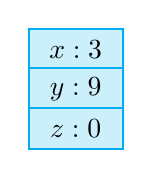
\begin{tikzpicture}
				\node[
					entries
				] (sm1) {$x : 3$};
				%
				\node[
					entries,
					anchor=north,
					yshift=\logentrieslinewidth
				] (sm2) at (sm1.south) {$y : 9$};
				%
				\node[
					entries,
					anchor=north,
					yshift=\logentrieslinewidth
				] (sm3) at (sm2.south) {$z : 0$};
				%
			\end{tikzpicture}
		};
		
		% Consensus Module
		\node[
			replicated,
			anchor = west,
			shift={(\padding,0)},
		] (consensus module) at (server\numservers.west|-state machine.west) {consensus\\module};	

		% Client
		\coordinate (client) at (-3,0|-consensus module);
		
		\foreach \i in {1,...,\numclients} {
			\pgfmathsetmacro{\displacement}{\i * \deltadimclient}
			\node[
				client,
			] (client\i) at ($(client) + (-\displacement,\displacement)$) {client};
		}
		
		% Arrows
		%% client -> consensus module
		\draw[connection] (client\numclients)
									 to[out=50, in=150] 
									 node[node_label, shift={(0,-\connectionshift)}] {1}
						  (consensus module);
		%% consensus module -> log
		\draw[connection] (consensus module) 
									to[out=270, in=140] 
									node[node_label, shift={(-\connectionshift,0)}] {2} 
						  (log);
		%% log -> state machine
		\draw[connection] (log) 
									to[out=0, in=300] 
									node[node_label, pos=0.7, shift={(\connectionshift,0)}] {3} 
						  (state machine);
		%% state machine -> client
		\draw[connection] (state machine) 
									to[out=140, in=70] 
									node[node_label, shift={(0,\connectionshift)}] {4} 
						  (client\numclients);
		%% consensus module -> server
		\foreach \i in {1,...,\numservers} {
			\ifnum\i=\numservers\else 
			\draw[connection] (consensus module) 
										to[out=190, in=195, looseness=1.5] 
										node[shift={(-\connectionshift,0)}] (server_node\i) {} 
							  (server\i.south west);
			\fi
		}
		%%% Label
		\node[
			node_label
		] at (server_node1) {2};
	\end{tikzpicture}
\end{document}